\section{Signal and background modelling of \texorpdfstring{\mgg}{myy}}
\label{sec:signalbackgroundmodelling}
The numbers of signal and background events in data are estimated with a fit to the \mgg spectrum as described in Section~\ref{sec:signalyieldextraction}. The functional form used to model the signal component is described in Section~\ref{ssec:signal_model}.
The forms used for the background are described in Section~\ref{ssec:background_model}.

\subsection{Signal Modelling}
\label{ssec:signal_model}
The \mgg distribution for the signal process $pp\rightarrow H \rightarrow\gamma\gamma$ is resonant.
In the absence of interference with the $pp\rightarrow\gamma\gamma$ background process this is expected to follow a Breit-Wigner curve, which peaks at the Higgs mass $m_H$ and in the Standard Model has a narrow width of $4~\text{MeV}$.
However, the distributions observed in data are smeared by the finite resolution of the measured photon energies.
For this reason, the \mgg distribution is modelled by fitting a double-sided Crystal Ball to the MC simulation with ${m_H = \SI{125}{\GeV}}$.
%% described in the common note\CiteCommon.
The analytic form of this function is presented in Eq.~\ref{E. DSCB}
\begin{equation}
  \begin{aligned}
    CB(\mgg) = N \times
    \begin{cases}
      e^{-t^{2}/2}, & \text{if } -\alpha_\text{low} \leq t \leq \alpha_\text{high} \\
      e^{-{}^{1}_{2} \alpha_\text{low }^{2}} \Big[ \frac{1}{R_\text{low}} \big(R_\text{low} - \alpha_\text{low} - t \big) \Big]^{-n_\text{low}},     & \text{if } t < -\alpha_\text{low} \\
      e^{-{}^{1}_{2} \alpha_\text{high}^{2}} \Big[ \frac{1}{R_\text{high}} \big(R_\text{high} - \alpha_\text{high} - t \big) \Big]^{-n_\text{high}}, & \text{if } t > \alpha_\text{high} \\
    \end{cases}
    \label{E. DSCB}
  \end{aligned}
\end{equation}

where $t=(\mgg-\mu_\text{CB})/\sigma_\text{CB}$, $R_\text{low}=\frac{\alpha_\text{low}}{n_\text{low}}$, and $R_\text{high}=\frac{\alpha_\text{high}}{n_\text{high}}$.
Here $N$ is a normalization parameter, $\mu_\text{CB}$ is mean of the Gaussian distribution, $\sigma_\text{CB}$ is the width of the Gaussian distribution, $\alpha_\text{low}$ and $\alpha_\text{high}$ are the positions of the transitions from the Gaussian core to the exponential tails on the low and high mass sides, and $n_\text{low}$ and $n_\text{high}$ are the exponents of the low and high mass tails.An example of this shape is shown in Figure~\ref{F. DSCB}.
The shape parameters are common to all processes ($ggH$, $VBF$, $VH$, $ttH$, $bbH$), and a fit to the sum of all processes normalised to their expected SM yield is performed for each inclusive region or bin of the differential variables.

\begin{figure}[htb!]
  \begin{center}
    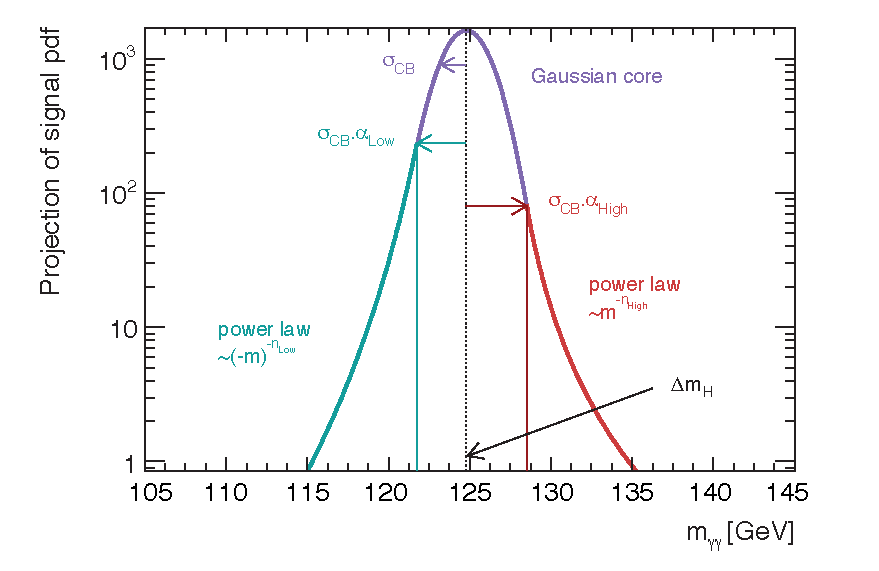
\includegraphics[width=0.48\textwidth]{figures/signal_modeling/DSCB.pdf}
  \end{center}
  \caption{Example of a double-sided crystal ball function.}
  \label{F. DSCB}
\end{figure}

Each of the shape parameters is determined by performing a fit to simulated ${H\to\gamma\gamma}$ decays at ${\mgg=\SI{125}{\GeV}}$.
In order to simulate a Higgs boson with a mass of 125.09\,\GeV, the resulting $\mu_\textrm{CB}$ will be shifted by 90\,\MeV.
This value is then fixed in the signal extraction fit and can vary for the different bins.
Shifts in $\mu_\textrm{CB}$ are still allowed through uncertainties taken into account as nuisance parameters in the fit, described in the next section.
This parametrisation is derived separately for each bin (aka category) of the variable in question.
Figures~\ref{Signal Param Inclusive Fiducial} show an example of fits for the inclusive fiducial volume.
Signal modelling plots for the other fiducial volumes and for the differential variables are shown in Appendix \ref{app:signal_fit}.
\begin{figure}[htb!]
  \begin{center}
        \includegraphics[width=0.48\textwidth]{figures/signal_modeling/fit_plots_Diphoton_fid_bin1.png}
  \end{center}
  \caption{Signal parametrisation for the inclusive fiducial volume normalised to 168~\ifb\
  }
  \label{Signal Param Inclusive Fiducial}
\end{figure}

\subsection{Background Modelling }
\label{ssec:background_model}

The main backgrounds in this analysis are non-resonant continuum backgrounds from inclusive $\gamma-\gamma$, $\gamma-jet$ and $jet-jet$ events.
These have smoothly falling distributions and are described by an empirically chosen functional form.
This may cause an increase (or decrease) in the measured signal events, so the selection is based on picking the function separately for each bin which reduces this bias, as described in Section~\ref{SSS. Spurious signal}.
Several functional forms for parametrization of the diphoton mass spectrum background were considered: exponentials of first (Exp), second (ExpPoly2), and third (ExpPoly3) degree polynomials, Bernstein polynomials of degree 3 (Bern3), 4 (Bern4), and 5 (Bern5) and power law functions of first (Pow)  order.
Previous studies \cite{ATLAS_prevNote} showed that the best function to model the background distribution in most cases is ExpPoly2:
\begin{equation}
  \mathcal{B}\left(\mgg;\textbf{$\alpha^\text{bkg}$}\right) = N\left(\textbf{$\alpha^\text{bkg}$}\right) \cdot \exp \left( - \frac{\mgg}{\alpha_1^\text{bkg}} - \frac{m_{\gamma\gamma}^2}{\alpha_2^\text{bkg}} \right)
\end{equation}
where $\alpha^\text{bkg}_{1}$, $\alpha^\text{bkg}_{2}$ are nuisance parameters and $N\left(\textbf{$\alpha^\text{bkg}$}\right)$ normalises the function to unity.
In general, a higher-order exponential is needed for bins with more events.

The Bernstein polynomials of degree $n$ are defined as:
\begin{equation}
   \mathcal{B}\left(\mgg;\textbf{$\alpha^\text{bkg}$}\right) = N\left(\textbf{$\alpha^\text{bkg}$}\right) \cdot
   \sum_{i=0}^n \alpha^\text{bkg}_i x^{i} \cdot (1 - x)^{n-i} \cdot \frac{n!}{i! \cdot (n-i)!}
\end{equation}

where $x = \frac{\mgg-\mgg^\textrm{min}}{\mgg^\textrm{max}-\mgg^\textrm{min}}$ is a variable defined in the range $[0,1]$ and $\alpha^\text{bkg}_0=1$.

For the power law function, the first order (Pow) is defined as

\begin{equation}
  \mathcal{B}\left(\mgg;\textbf{$\alpha^\text{bkg}$}\right) = N\left(\textbf{$\alpha^\text{bkg}$}\right) \cdot m_{\gamma\gamma}^{\alpha_1}
\end{equation}


\FloatBarrier

\subsubsection{Spurious signal} 
\label{SSS. Spurious signal}

The spurious signal method is used to measure the bias in the signal yield caused by the choice of background parameterisation.
This is done by fitting a background only MC simulation with a signal + background parameterisation. 
Due to computational limitations only the $\gamma\gamma$ sample is generated, the contribution of $\gamma j$ and $jj$ component are derived from data using a two-dimensional
double-sideband method described in \ref{sec:backgroundestimation}.The fraction of contributed by the $\gamma\gamma$,$\gamma j$ and $jj$ background source after inclusive diphoton selection are 67\%,29\% and 4\% respectively. In ~\cite{ATLAS_prevNote},it was studied that using only $\gamma\gamma$ and $\gamma j$ components for modelling the shape, a good description of the background in the data sideband can be achieved and the $jj$ contribution can be neglected.For each bin 
A background-only template is build as the sum of $\gamma\gamma$ and $\gamma j$ components according to the relative fractions measured with data.The total template is then normalised to match the data sideband. 

Due to the finite size of the simulation samples used to build the background templates,
large statistical fluctuations are often observed. These fluctuations can adversely affect
the estimation of the spurious signal, particularly when they occur in the Higgs signal
window between 123\GeV and 127 \GeV. These fluctuations would nominally be interpreted
as a spurious signal, hence resulting in an overestimation of the background model’s
systematic uncertainty. Given the computational limitations in generating larger data
sets, an alternative approach is employed. The background templates are smoothed using
Gaussian process regression (GPR) ~\cite{frate2017modelingsmoothbackgroundsgeneric},using the Gibbs Kernel. The GPR approach
suppresses statistical fluctuations in the background templates, without biasing the shape of wider features in the template.

The signal yield extracted in the background-only template (S) and its statistical uncertainty ($\Delta_{\textrm{S}}$) are used to measure the bias introduced by the choice of the background parametrisation. The condition of a function to be accepted is that either:

\begin{itemize}
	\item S  is less than 20\% of the background uncertainty
	\item S  is less than 10\% of the number of expected signal events.
\end{itemize}


The mass range of 123-127\,\GeV\ is split into  bins with a 0.5\,\GeV\ width and the maximal signal found in these bins is taken as spurious signal.
 
In case several functions satisfy the above criteria, the one with fewest degree of freedom is chosen. If two such functions are found , the one with the lower spurious signal uncertainty is taken. 
 
Furthermore, an additional  $\chi^2$ probability ensures that the side-bands from the  MC templates are also described well requiring that the $p$-value is larger than 1\%. 
